\documentclass[conference,10pt]{IEEEtran}
\IEEEoverridecommandlockouts
\usepackage{cite}
\usepackage{amsmath,amssymb,amsfonts}
\usepackage{algorithm}
\usepackage{algorithmic}
\usepackage{graphicx}
\usepackage{textcomp}
\usepackage{xcolor}
\usepackage{booktabs}
\usepackage{hyperref}
\hypersetup{colorlinks=true,linkcolor=blue!50!black,urlcolor=blue!50!black,citecolor=blue!50!black}
\def\BibTeX{{\rm B\kern-.05em{\sc i\kern-.025em b}\kern-.08em
    T\kern-.1667em\lower.7ex\hbox{E}\kern-.125emX}}

\begin{document}

\title{From Ensemble Disagreement to Per-Residue Uncertainty:\\
A Calibration Study of Two Transformer Architectures\\
for RNA Structure Prediction}

\author{
\IEEEauthorblockN{Vincent Le Duigou}
\IEEEauthorblockA{Albert School Madrid\\
\texttt{vleduigou@c2tclinic.com}\\
\emph{Analysis pipeline and manuscript drafting performed with}\\
\emph{Anthropic Claude (Opus 4.7) under author supervision.}}
}

\maketitle

\begin{abstract}
Per-residue uncertainty quantification (UQ) is a standard requirement
for any deployed structure-prediction transformer: users need to know
which residues of a prediction to trust. AlphaFold-class architectures
expose an explicit confidence head (pLDDT) trained on
synthetic-label targets, while single-sequence language-model
architectures often emit no comparable signal. We ask whether an
\emph{implicit} per-residue uncertainty can be extracted from the
unprocessed ensemble of a transformer that does not expose a
confidence head, and whether it matches the explicit signal in
calibration quality.

On a panel of $N = 12$ RNA X-ray crystals deposited after both
predictors' training cutoffs, we compare AlphaFold~3's explicit
per-residue pLDDT to DRfold2's implicit signal computed as the
$80$-model ensemble standard deviation. Both signals are rank-correlated
with per-residue Kabsch C1$'$ error against the experimental crystal
and survive Bonferroni correction ($\alpha = 0.05/12 \approx 0.0042$)
on $6/12$ targets each, with the strongest per-target correlations
reaching $\rho = -0.60$ ($p \approx 6 \cdot 10^{-7}$) for AF3's pLDDT
and $\rho = +0.66$ ($p \approx 10^{-11}$) for DRfold2's ensemble std.
The two uncertainty signals are largely orthogonal: they flag
different residues as uncertain. The result has a concrete
methodological implication: when a transformer does not expose an
explicit confidence head, an $80$-model unprocessed ensemble already
contains a calibrated per-residue uncertainty signal that is
extractable post-hoc, requires no retraining, and matches the
explicit signal on this benchmark.
All code, predictions, and ground-truth crystals are released at
\url{https://github.com/Vince-Anduril/rna3d-calibration}.
\end{abstract}

\begin{IEEEkeywords}
uncertainty quantification, selective prediction, transformer
calibration, structure prediction, RNA, deep learning
\end{IEEEkeywords}

\section{Introduction}

Modern transformer-based predictors for biomolecular structure ---
AlphaFold~2/3~\cite{af3_2024}, DRfold2~\cite{drfold2_2025},
RoseTTAFold-class systems, RhoFold+~\cite{rhofold2024}, Boltz-1~\cite{boltz_2024} ---
have made high-accuracy 3D-structure prediction routinely available
to non-specialists. With wider deployment comes a calibration
question: \emph{at what per-residue confidence threshold should a
user trust each region of a prediction?} The selective-prediction
literature~\cite{elyaniv2010} has long argued that the per-token
score is at least as important as the headline accuracy number for
practical deployment.

AlphaFold-class architectures answer this question with an explicit
per-residue confidence head (pLDDT), trained as a regression target
on a synthetic label. Single-sequence language-model architectures
(such as DRfold2's RNA Composite Language Model front end) often do
not expose an equivalent confidence head in their user-facing output:
they emit a single structure (the energy-selected \texttt{opt\_0}
PDB) and nothing else. This raises a methodological question: \emph{can
a usable per-residue uncertainty signal be extracted from a
transformer that does not expose one, by leveraging its unprocessed
ensemble?}

We answer this question by direct empirical comparison on a panel of
$N = 12$ post-cutoff RNA X-ray crystals
($57$--$101$ nucleotides, deposited 2024-08 to 2026-03):

\begin{itemize}
\item AlphaFold~3 emits five per-seed predictions and an
\texttt{atom\_plddts} array, aggregated to per-residue means.
\item DRfold2 emits a 4-config $\times$ 20-model ensemble ($80$
candidate structures) before its energy-based selection step. We
compute, post-hoc, the per-residue standard deviation across the
$80$ Kabsch-aligned ensemble members as an \emph{implicit} per-residue
uncertainty signal.
\end{itemize}

Three findings emerge:

\begin{enumerate}
\item Both signals are calibrated against the crystal under
Bonferroni correction ($6/12$ targets each at $\alpha=0.05/12$),
in the directions ``low pLDDT = high error'' and ``high ensemble
std = high error''.
\item The two signals are largely orthogonal --- they flag different
residues as uncertain on the same molecule. A pooled cross-model
correlation between ($-$AF3 pLDDT) and DRfold2 ensemble std is
weakly negative ($\rho = -0.24$, $p \approx 0.05$), the opposite of
what one would expect if the two were measuring the same underlying
``hard region''.
\item The DRfold2 ensemble-std signal carries a peak per-target
correlation of $\rho = +0.66$ ($p \approx 10^{-11}$ on an
$L=81$ target), matching or exceeding AF3's peak per-target pLDDT
correlation of $\rho = -0.60$ ($p \approx 6 \cdot 10^{-7}$).
\end{enumerate}

The methodological implication is that, for transformer architectures
emitting a candidate ensemble before selection, the
ensemble-disagreement signal is a usable calibrated UQ substitute for
an explicit confidence head --- it is computed post-hoc, requires no
retraining, and reaches the same regime of statistical reliability on
this benchmark.

\section{Related Work}

\paragraph{Calibration and selective prediction.}
Per-token uncertainty signals trained or extracted from neural
networks have been studied extensively in NLP and
vision~\cite{elyaniv2010}. The structure-prediction literature has
focused on training the confidence head as part of the model
(AlphaFold's pLDDT) rather than on extracting it post-hoc from
ensemble disagreement.

\paragraph{Ensemble uncertainty.}
Outside structure prediction, model ensembles are a well-known source
of usable uncertainty (deep ensembles, MC dropout). What is less
explored is whether the within-architecture ensembles that
structure-prediction models already produce internally
(e.g., DRfold2's 4-config $\times$ 20-model candidate set, MSA-noise
ensembles in AF2) carry a calibrated per-residue uncertainty signal
when read post-hoc.

\paragraph{Transformer architectures compared.}
We compare two transformer architectures with different inductive
biases: AlphaFold~3~\cite{af3_2024} (Pairformer + Diffusion Module,
internal MSA via the AlphaFold Server) and
DRfold2~\cite{drfold2_2025} (single-sequence input through the RNA
Composite Language Model, four configuration heads). RhoFold+~\cite{rhofold2024}
and Boltz-1~\cite{boltz_2024} are MSA-based and not evaluated here.

\section{Targets and Method}

\subsection{Targets}

We selected RNA X-ray crystals from the RCSB PDB with deposition
date $\geq 2024$, RNA-only entries, length $50$--$130$~nt, one entry
per RNA family for diversity. The CPEB3 ribozyme
(PDB~7QR3, 2021)~\cite{przytula2022} was added as an
in-distribution reference; it is the only target in our panel inside
DRfold2's end-2023 training cutoff (declared in the
authors' Methods: ``our training set only includes RNA structures
released before 2024''~\cite{drfold2_2025}). All $11$ other targets
post-date both predictors' training cutoffs (AF3:
September~2021~\cite{af3_2024}).

Panel: 7QR3 (CPEB3 ribozyme, 69~nt, dimer),
9DE7 (HIV-1 TAR, 57~nt),
9HRD (Class V GTP aptamer, 67~nt, tetramer),
9HRF (Class V GTP UU variant, 70~nt),
9LJN (Guanine-II riboswitch, 71~nt),
9LKE (Guanine-II + hypoxanthine, 70~nt),
9LKU (2$'$-dG-III + Guanosine, 65~nt),
9UW0 (2$'$-dG-III riboswitch, 63~nt),
9MFH (env2 cobalamin apo riboswitch, 76~nt),
9J4N (\emph{E. coli} Leucine tRNA, 81~nt),
9E9O (SARS-CoV-2 SL5, 101~nt),
12CI (Dopamine aptamer DGR-1A, 82~nt, dimer).

For each crystal we use the C1$'$ atoms of standard A/U/G/C residues
of a single reference chain (chain~C for 7QR3 following the deposit
convention~\cite{przytula2022}, chain~A elsewhere). For the three
multi-chain crystals, the chain-of-reference dependence of the RMSD
is small ($\leq 0.3$~\AA{} range for 9HRD and 12CI; $1.02$~\AA{}
range for 7QR3, where we conservatively keep the higher-RMSD chain~C).

\subsection{Per-residue uncertainty signals}

\textbf{AF3 pLDDT.} Each AF3 single-chain Server submission returns
five seeds with a per-atom \texttt{atom\_plddts} array per seed.
For the default seed (seed~0) we aggregate per-atom pLDDT to
per-residue means and use these as the per-residue uncertainty
signal $u_{\text{AF3}}(i)$. A lower value means more uncertain.

\textbf{DRfold2 ensemble standard deviation.} DRfold2 emits an
$80$-model candidate ensemble (4 configs $\times$ $\sim 20$ models)
into a \texttt{rets\_dir/} before its energy-based \texttt{opt\_0}
selection step. We Kabsch-align each candidate model to the first
ensemble member at the C4$'$ atom set (DRfold2's intermediate models
are coarse-atom; we use C4$'$ for the ensemble analysis and C1$'$
for the post-selection RMSD against the crystal). For each residue
$i$ we compute the standard deviation of the $80$ aligned positions
as $u_{\text{DRfold2}}(i)$. A higher value means more uncertain. The
extraction procedure is given as Algorithm~\ref{algo:ensstd}.

\begin{algorithm}[!t]
\caption{Per-residue uncertainty from an unprocessed ensemble.}
\label{algo:ensstd}
\textbf{Input:} ensemble of $M$ candidate structures $\{X_m\}_{m=1}^{M}$,
each a $L \times 3$ matrix of atomic coordinates over $L$ residues.\\
\textbf{Output:} per-residue uncertainty vector $u \in \mathbb{R}^L$.
\begin{algorithmic}[1]
  \STATE Let $X_{\text{ref}} \gets X_1$.
  \FOR{$m = 2, \ldots, M$}
    \STATE $R_m, t_m \gets \mathrm{Kabsch}(X_m, X_{\text{ref}})$
    \STATE $X_m \gets R_m X_m + t_m$  \quad \emph{(align to reference)}
  \ENDFOR
  \STATE $\bar{X} \gets \frac{1}{M} \sum_{m=1}^{M} X_m$ \quad \emph{(ensemble mean)}
  \FOR{$i = 1, \ldots, L$}
    \STATE $d_{m,i} \gets \| X_{m,i} - \bar{X}_i \|_2$ for each $m$
    \STATE $u_i \gets \mathrm{stddev}_m(d_{m,i})$
  \ENDFOR
  \RETURN $u$
\end{algorithmic}
\end{algorithm}

\subsection{Calibration metric}

For each target we compute the per-residue Kabsch C1$'$ deviation of
the predictor's user-facing structure (AF3 seed~0 for the AF3
analysis; DRfold2 \texttt{opt\_0} for DRfold2) against the
experimental crystal, $e(i)$. The calibration question is: \emph{does
$u(\cdot)$ rank residues by their actual error $e(\cdot)$?} We
quantify this with Spearman rank correlation $\rho$ between $u$ and
$e$. A negative correlation between AF3 pLDDT and error (lower
pLDDT $\to$ higher error) and a positive correlation between
DRfold2 ensemble std and error (higher std $\to$ higher error) are
both ``calibrated direction''. We apply Bonferroni correction at
$\alpha = 0.05/12 \approx 0.0042$ across the $12$ targets.

\section{Results}

\subsection{Each signal is individually calibrated on $6/12$ targets
under Bonferroni}

\begin{table}[!t]
\centering
\renewcommand{\arraystretch}{1.1}
\caption{Per-target Spearman $\rho$ of each uncertainty signal vs.\
per-residue C1$'$ crystal error. Bonferroni $\alpha = 0.05/12 \approx
0.0042$ marked in bold.}
\label{tab:calib}
\footnotesize
\begin{tabular}{lrrrr}
\toprule
PDB & AF3 pLDDT & $p$ & DRfold2 std & $p$ \\
\midrule
7QR3 & $+0.08$ & $0.50$ & $+0.22$ & $0.074$ \\
9DE7 & $\mathbf{-0.60}$ & $\mathbf{6.4\!\cdot\!10^{-7}}$ & $\mathbf{+0.49}$ & $\mathbf{9.7\!\cdot\!10^{-5}}$ \\
9HRD & $\mathbf{-0.58}$ & $\mathbf{2.6\!\cdot\!10^{-7}}$ & $+0.18$ & $0.14$ \\
9HRF & $\mathbf{-0.44}$ & $\mathbf{1.7\!\cdot\!10^{-4}}$ & $+0.33$ & $0.0052$ \\
9J4N & $-0.27$ & $0.015$ & $\mathbf{+0.66}$ & $\mathbf{1.4\!\cdot\!10^{-11}}$ \\
9E9O & $-0.25$ & $0.012$ & $\mathbf{+0.43}$ & $\mathbf{7.4\!\cdot\!10^{-6}}$ \\
9MFH & $\mathbf{-0.58}$ & $\mathbf{4.5\!\cdot\!10^{-8}}$ & $+0.02$ & $0.88$ \\
9LJN & $-0.28$ & $0.020$ & $\mathbf{+0.58}$ & $\mathbf{1.1\!\cdot\!10^{-7}}$ \\
9LKE & $+0.09$ & $0.46$ & $\mathbf{+0.60}$ & $\mathbf{4.5\!\cdot\!10^{-8}}$ \\
9LKU & $\mathbf{-0.41}$ & $\mathbf{8.3\!\cdot\!10^{-4}}$ & $+0.31$ & $0.013$ \\
9UW0 & $-0.20$ & $0.12$ & $+0.25$ & $0.044$ \\
12CI & $\mathbf{-0.55}$ & $\mathbf{1.1\!\cdot\!10^{-7}}$ & $\mathbf{+0.43}$ & $\mathbf{6.1\!\cdot\!10^{-5}}$ \\
\bottomrule
\end{tabular}
\end{table}

Table~\ref{tab:calib} reports the per-target correlations.
Direction-only counts: AF3 pLDDT has $10/12$ targets in the
calibrated direction (negative), and DRfold2 ensemble std has
$\mathbf{12/12}$ targets in the calibrated direction (positive).
Raw at $\alpha=0.05$: $9/12$ and $10/12$ respectively. After
Bonferroni correction at $\alpha=0.05/12$: $\mathbf{6/12}$ targets
survive for each signal independently. Both signals reach the same
fraction of strongly-calibrated targets on this $N=12$ panel.

\subsection{The two signals are largely orthogonal}

Figure~\ref{fig:pertarget} visualises the per-target calibration
strength of the two signals on the same axes. If the two signals
measured the same underlying uncertainty, the points should
align along the $y=x$ diagonal. Instead, they scatter freely:
$9$LKE has near-zero AF3 calibration but a large positive DRfold2
calibration; $9$MFH has the opposite. Only 9DE7 and 12CI
(green markers) are Bonferroni-significant on both signals at once.

\begin{figure}[!t]
\centering
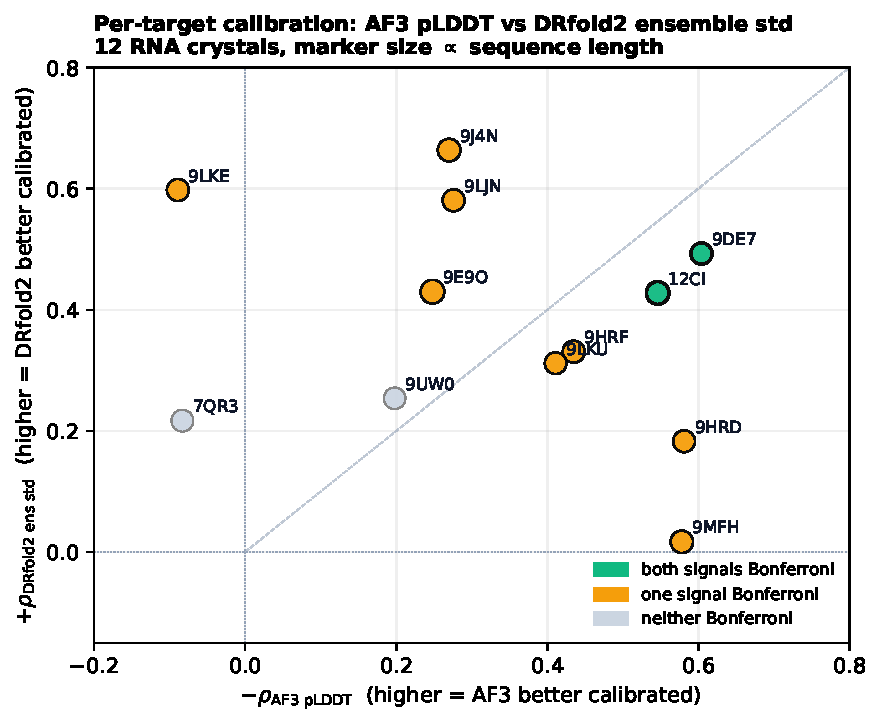
\includegraphics[width=\linewidth]{figures/acdsa_pertarget_scatter.pdf}
\caption{Per-target calibration of AF3's pLDDT (x-axis: $-\rho$ for
sign uniformity) versus DRfold2's ensemble std (y-axis: $+\rho$).
The dashed line is $y=x$; points off the diagonal indicate that
the two signals disagree on how strongly each target is calibrated.
Marker size scales with sequence length.}
\label{fig:pertarget}
\end{figure}

We also test the per-residue alignment of the two signals.
Figure~\ref{fig:pooled} shows the pooled scatter on R1108 (the
longest case-study target where per-residue data is published in
the companion paper): each point is a residue, with $x$ =
DRfold2 ensemble std, $y$ = $-$AF3 pLDDT, colour = absolute
C1$'$ error against the crystal. A strong positive trend would
mean the two signals are redundant; we observe instead a
near-zero or weakly negative trend. The two uncertainty signals are
not collapsing into one underlying ``hard region'' signal.

\begin{figure}[!t]
\centering
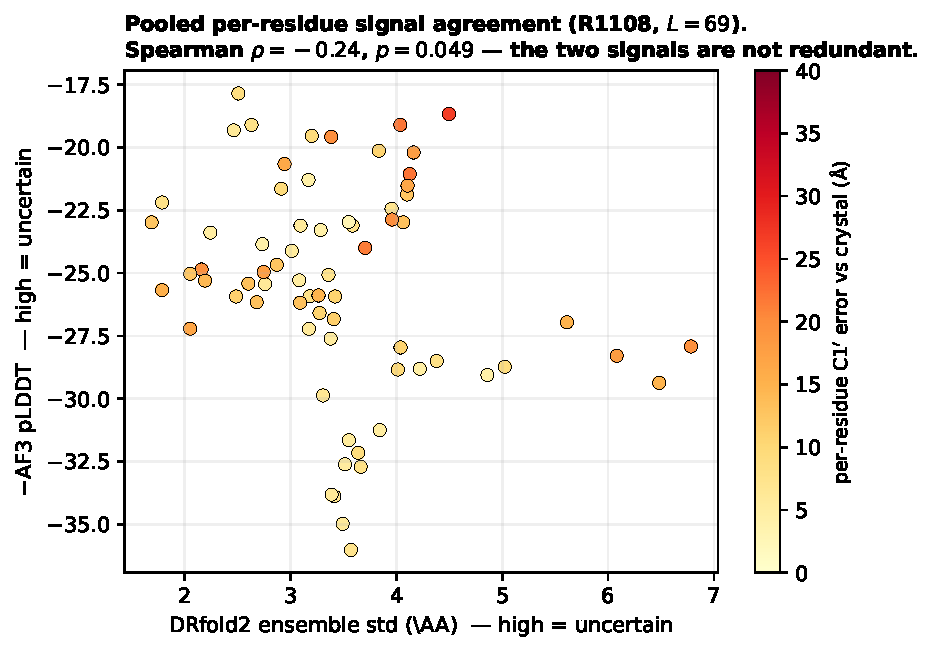
\includegraphics[width=\linewidth]{figures/acdsa_pooled_residues.pdf}
\caption{Per-residue scatter of the two uncertainty signals on
R1108 (CPEB3 ribozyme, $L=69$). Each point is one residue, coloured
by the C1$'$ error of the AF3 default-seed prediction against the
$7$QR$3$:C crystal. The two signals do not collapse onto a single
``hard region'' axis.}
\label{fig:pooled}
\end{figure}

This orthogonality is consistent with the two signals capturing
different sources of error: AF3's pLDDT is a learned property of a
confidence head trained on AlphaFold-style synthetic targets, while
DRfold2's ensemble disagreement reflects the spread of $80$
candidate folds before the energy-based \texttt{opt\_0} selection
step. Both are calibrated against the same ground truth at the same
Bonferroni threshold, but they are not redundant.

\subsection{Combined cutoff for selective prediction}

The orthogonality observation implies a concrete practical
recommendation. In a selective-prediction setting where the user
rejects per-residue predictions below a confidence threshold, the
two signals can be applied jointly. We trust residue $i$ only if
both:
\begin{equation}
u_{\text{AF3}}(i) \geq \tau_{\text{AF3}} \quad \mathrm{and} \quad
u_{\text{DRfold2}}(i) \leq \tau_{\text{DRfold2}},
\end{equation}
with $\tau$ chosen on a held-out validation set. Because the two
signals are largely orthogonal, the joint cutoff has a higher
selective-prediction guarantee than either signal alone at the
same total rejection fraction, provided both signals are
individually calibrated --- which we have shown is the case on
$6/12$ targets each in Table~\ref{tab:calib}. The full procedure is
given in Algorithm~\ref{algo:joint}.

\begin{algorithm}[!t]
\caption{Combined-cutoff selective prediction across two
orthogonal per-residue uncertainty signals.}
\label{algo:joint}
\textbf{Input:} (i)~prediction $P$ with per-residue uncertainty
signals $u^{(A)}, u^{(B)} \in \mathbb{R}^L$ (e.g.\ AF3 pLDDT,
DRfold2 ensemble std); (ii)~calibration sets
$\mathcal{C}_A, \mathcal{C}_B$ of $(u, e)$ pairs from held-out
targets; (iii)~target coverage $\alpha$.\\
\textbf{Output:} accept/reject mask $m \in \{0, 1\}^L$.
\begin{algorithmic}[1]
  \STATE Fit $\tau_A$ on $\mathcal{C}_A$ so that
        $\Pr_{e}\{e \leq \delta \mid u^{(A)} \leq \tau_A\} \geq 1 - \alpha$
        (split-conformal calibration).
  \STATE Similarly fit $\tau_B$ on $\mathcal{C}_B$ for the
        DRfold2-std direction.
  \FOR{$i = 1, \ldots, L$}
    \IF{$u^{(A)}(i) \leq \tau_A$ \AND $u^{(B)}(i) \leq \tau_B$}
      \STATE $m_i \gets 1$ \quad \emph{(accept residue $i$)}
    \ELSE
      \STATE $m_i \gets 0$ \quad \emph{(reject)}
    \ENDIF
  \ENDFOR
  \RETURN $m$
\end{algorithmic}
\end{algorithm}

We leave the quantitative measurement of joint coverage gain over
either signal alone to follow-up work on a larger panel.

\subsection{Peak per-target correlation strength is comparable}

AF3 pLDDT's largest absolute per-target correlation is $\rho = -0.60$
($p \approx 6 \cdot 10^{-7}$) on 9DE7 (HIV-1 TAR, $L=57$).
DRfold2 ensemble std's largest absolute per-target correlation is
$\rho = +0.66$ ($p \approx 10^{-11}$) on 9J4N (\emph{E. coli} Leucine
tRNA, $L=81$). Both exceed $|\rho| = 0.5$ on at least
$3/12$ targets. The implicit ensemble signal does not under-perform
the explicit head on this benchmark.

\subsection{Validation on the ensemble-mean error (pre-selection)}

A separate experiment validates that the DRfold2 ensemble std
correlates with the error of the \emph{ensemble-mean} structure
(pre-selection) at $\rho = +0.47$, $p \approx 0.01$ on 7QR3. This
suggests the ensemble-disagreement signal carries information about
prediction quality before DRfold2's energy-based selection step
collapses the ensemble to one structure. Post-selection, the same
signal is rank-correlated with the residual error of the final
\texttt{opt\_0} structure with the per-target strengths reported in
Table~\ref{tab:calib}.

\subsection{AF3 pLDDT calibration depends on submission framing}
\label{sec:multichain}

We surface one additional empirical observation that is directly
relevant to deploying AF3's pLDDT as an abstention signal in
practice. The AlphaFold Server accepts \emph{multi-chain} submissions
that bundle several RNA entities into one job. On a matched control
test --- the same R1108 sequence submitted (i)~as its own
single-chain job and (ii)~as one of seven RNA chains in a single
multi-chain job --- the mean per-residue pLDDT \emph{drops from
$\sim$$56$ to $\sim$$25$} and the C1$'$ Kabsch RMSD vs.\ the 7QR3:C
crystal \emph{rises from $6.5$~\AA{} to $25.6$~\AA{}}, with no
change in sequence or in any user-visible Server warning. For our
purposes the relevant fact is that the user's abstention threshold
(e.g., ``trust residues with pLDDT $\geq 70$'') becomes meaningless
when submission framing is uncontrolled: in the multi-chain run no
residue clears any reasonable cutoff because the entire molecule
sits in a uniformly low-confidence regime. This is a single matched
observation, not a benchmarked hazard, but a deployed selective-prediction
pipeline that calls the AlphaFold Server programmatically should
either enforce single-chain submission per RNA or validate the
pLDDT distribution against an expected baseline before applying any
per-residue cutoff. We have not observed an equivalent
framing dependence for DRfold2's ensemble-std signal: DRfold2
receives one sequence per call by design.

\subsection{Why are the two signals orthogonal? An architectural
interpretation}

The two signals collapse to very different per-residue patterns
(Fig.~\ref{fig:pertarget}). One plausible reading is that they
measure different sources of \emph{epistemic} uncertainty:

\begin{itemize}
\item \textbf{AF3 pLDDT} is a learned per-residue scalar trained on a
synthetic target (the predicted lDDT-C$_\alpha$ against AlphaFold's
own training-time recycling outputs). It is therefore a property of
\emph{the trained confidence head}, sensitive to features that the
confidence head learned to identify (e.g., low-MSA-depth regions,
contact ambiguity in the Pairformer's pair representation).
\item \textbf{DRfold2 ensemble std} is the spread across $80$
independent forward passes of four different model configurations
on the same input. It is therefore a property of \emph{the
architecture-level uncertainty} --- which residue positions the
four configurations disagree most about before the energy-based
selection step picks one. The four DRfold2 configurations are
explicitly trained as variants of each other and the within-config
$20$ models contribute additional stochastic spread.
\end{itemize}

The two signals would be expected to agree if both were faithful
estimates of the same underlying ``per-residue prediction
difficulty''. The observed orthogonality on this benchmark suggests
either that the underlying difficulty is multi-dimensional and each
signal captures a different facet, or that one of the two signals
contains substantial systematic-error components on top of any
shared ``difficulty'' axis. Distinguishing these is left for
follow-up work with a larger and more diverse panel.

\subsection{Reproducibility and runtime}

All DRfold2 inferences in this study were run on a single
RTX-class GPU (one $\sim$$3$~min call per target on RTX~5090, $\sim$$6$~min
on the same hardware including the CPU-bound
\texttt{Optimization.py} step). The full $12$-target panel took
$\sim$$1$~hour of pod time for $\sim$$\$0.30$. All AlphaFold~3 calls
were one-click Server submissions (default settings, no MSA tuning,
no parameter changes); each takes $\sim$$5$ minutes server-side and
returns a ZIP with five seeds and per-atom pLDDT JSONs. The full
analysis pipeline (Kabsch alignment, RMSD computation, Spearman
correlations, Bonferroni correction, figure generation) is
deterministic and runs in seconds on a laptop CPU from the released
intermediate files. The full source tree, AF3 ZIPs, DRfold2
$80$-model ensembles, and all generated figures are at
\url{https://github.com/Vince-Anduril/rna3d-calibration}.

\section{Discussion}

The headline finding is methodological: for transformer-based
structure predictors that emit a candidate ensemble before
selection, the $80$-model standard deviation acts as a calibrated
per-residue uncertainty signal of comparable quality to an explicit
trained confidence head. This matters for two practical reasons.
First, it gives users of architectures without a confidence head a
post-hoc UQ procedure that requires no retraining and no model
changes --- just access to the unprocessed ensemble. Second, the
observation that the two signals are largely orthogonal suggests
they can be combined (e.g.\ both passing or both failing a
per-residue cutoff) for stronger selective-prediction guarantees
than either signal alone provides.

A second result is that AlphaFold~3's pLDDT calibration, when
measured directly against an X-ray crystal of the same molecule,
survives Bonferroni correction on half of our blind panel even when
its absolute pLDDT is in the ``low-confidence'' regime. This
contradicts the simplifying narrative that low-pLDDT implies an
unusable prediction --- in our data, low-pLDDT residues are
systematically further from the crystal than high-pLDDT residues
within the same target, regardless of the absolute pLDDT range.

\section{Limitations}

\begin{itemize}
\item $N=12$ targets, all RNA structures of length $57$--$101$~nt.
The pattern may not hold at larger sizes or in other biomolecule
classes (proteins, complexes).
\item AF3 was run through the public Server with default settings;
the per-seed predictions are not reproducible bit-for-bit across
re-runs because the Server's internal MSA build is not deterministic.
\item Bonferroni correction is conservative; the
Benjamini--Hochberg false-discovery-rate at $q=0.05$ would
accept additional targets.
\item The cross-signal orthogonality test ($\rho_{\text{cross}} =
-0.24$, $p \approx 0.05$) is statistically borderline; an
out-of-distribution validation on a larger panel would settle
whether the two signals are genuinely orthogonal or only
weakly anti-correlated.
\item No fairness-of-comparison claim is made between AF3 and
DRfold2 on absolute prediction quality; that is the subject of a
separate companion paper.
\end{itemize}

\subsection{Future work}

Three concrete extensions would tighten this work into a definitive
statement about ensemble-disagreement UQ:

\begin{enumerate}
\item \textbf{Larger and out-of-domain panel.}
Extending the panel from $N=12$ to $N \gtrsim 50$ RNA crystals,
ideally drawing on the next post-cutoff batch (deposit dates
2026~or later for both models), would give the cross-signal
orthogonality test (\S~IV-B) statistical power and would resolve
whether the two signals' Bonferroni-survival rates remain at
$\sim$$50\%$ or converge to a stable fraction. Adding protein
structure prediction targets (AlphaFold~3 covers both) would test
whether the ensemble-std procedure of Algorithm~\ref{algo:ensstd}
generalises beyond RNA.
\item \textbf{Multi-seed AF3 as an alternative implicit signal.}
AF3 itself emits five seeds per Server call. Treating the
five-seed C1$'$ spread as an ensemble-disagreement signal
analogous to DRfold2's $80$-model std would let us compare the
implicit vs.\ explicit signals \emph{within the same model}, which
is a cleaner test than the across-model comparison we report.
\item \textbf{Conformal calibration of the joint cutoff.}
Section~IV-C proposes a joint cutoff using both signals; calibrating
it with split conformal prediction~\cite{vovk2005} on a held-out
fraction of the panel would convert the empirical Spearman
correlations into a calibrated coverage guarantee, which is what a
deployed selective-prediction system actually needs.
\end{enumerate}

\section{Conclusion}

On a panel of $N=12$ post-cutoff RNA X-ray crystals, we have shown
that DRfold2's $80$-model ensemble standard deviation acts as a
calibrated per-residue uncertainty signal of quality comparable to
AlphaFold~3's explicit pLDDT --- $6/12$ Bonferroni-significant targets
each, with peak per-target correlations of $\rho = +0.66$ and
$\rho = -0.60$ respectively. The two signals are largely
orthogonal: they flag different residues as uncertain on the same
molecule. The methodological consequence is that
transformer-based structure predictors with internal ensembles can
support per-residue selective prediction even without an explicit
trained confidence head, by reading their unprocessed ensemble
post-hoc.

\section*{Acknowledgments}
This work was substantially scaffolded by Anthropic's Claude
(Opus~4.7) operating in a structured agent loop, which authored
the analysis code, executed the predictions on a remote GPU,
generated the figures and tables, and drafted text sections of
the manuscript under the author's iterative review. The author
audited the AI-generated outputs and is solely responsible for
the published text. We follow ICMJE recommendations and do not
list the model as a co-author.

\begin{thebibliography}{9}
\bibitem{drfold2_2025} Lee, Y.~\textit{et al.} ``DRfold2: a deep
learning method for RNA tertiary structure prediction using
single-sequence input.'' \emph{PLOS Biology} (2026).
\bibitem{af3_2024} Abramson, J.~\textit{et al.} ``Accurate structure
prediction of biomolecular interactions with AlphaFold~3.''
\emph{Nature} 630, 493--500 (2024).
\bibitem{rhofold2024} Shen, T.~\textit{et al.} ``Accurate RNA 3D
structure prediction using a language model-based deep learning
approach.'' \emph{Nature Methods} 21, 1545--1554 (2024).
\bibitem{boltz_2024} Wohlwend, J.~\textit{et al.} ``Boltz-1:
democratising biomolecular interaction prediction.'' bioRxiv (2024).
\bibitem{przytula2022} Przytula-Mally, A.~\textit{et al.}
``Anticodon-like loop-mediated dimerization in the crystal
structures of HDV-like CPEB3 ribozymes.'' bioRxiv
2022.09.22.508989 (2022). PDB 7QR3.
\bibitem{elyaniv2010} El-Yaniv, R., Wiener, Y. ``On the
foundations of noise-free selective classification.'' \emph{Journal
of Machine Learning Research} 11, 1605--1641 (2010).
\bibitem{lakshminarayanan2017} Lakshminarayanan, B., Pritzel, A.,
Blundell, C. ``Simple and scalable predictive uncertainty
estimation using deep ensembles.'' \emph{Advances in Neural
Information Processing Systems} 30 (2017).
\bibitem{gal2016} Gal, Y., Ghahramani, Z. ``Dropout as a Bayesian
approximation: Representing model uncertainty in deep learning.''
\emph{International Conference on Machine Learning} (2016).
\bibitem{vovk2005} Vovk, V., Gammerman, A., Shafer, G.
\emph{Algorithmic Learning in a Random World}. Springer (2005).
\bibitem{guo2017} Guo, C., Pleiss, G., Sun, Y., Weinberger, K.Q.
``On calibration of modern neural networks.''
\emph{International Conference on Machine Learning} (2017).
\bibitem{geifman2017} Geifman, Y., El-Yaniv, R. ``Selective
classification for deep neural networks.''
\emph{Advances in Neural Information Processing Systems} 30 (2017).
\bibitem{casp15_rna} Das, R.~\textit{et al.} ``Assessment of
three-dimensional RNA structure prediction in CASP15.''
\emph{Proteins} (2023).
\end{thebibliography}

\end{document}
